\documentclass[10pt,twoside,twocolumn,a4paper]{article}

%% Default action is for double-blinded peer review where 
%% authors, address and acknowledgements sections are hidden 
%\usepackage[]{bpasts}
%% For accepted papers enable option "accepted" to deanonymize
%% your manuscript 
\usepackage[accepted]{bpasts}

\usepackage{t1enc}
\usepackage[utf8]{inputenc}
\usepackage{amsmath,amsfonts}

\usepackage{graphicx}
\usepackage{flushend}

\usepackage[colorlinks=true, allcolors=bpastsblue, pdfborder={0 0 0}]{hyperref}

%%%%%%%%%%%%%%%%%%%%%%%%%%%%%%%%%%%%%%%%%%%%%%%%%%%%%%%
%% HEADER OF THE ARTICLE (Change all fields)
\abtitle{Paper for BPASTS}
\title{Preparation of Papers for BPASTS}

\abauthor{Autor(s) Name Last Name}
\author{Author(s) Name Last Name$^{1}$$^{2}$\email{smith@university.edu.pl}}

\Address{$^1$ Affiliation \\ $^2$ Affiliation}

\Abstract{This electronic document is a ``live'' template and already defines the components of your paper [title, text, heads, etc.] in its style sheet. The abstract must be written as one paragraph. An informative and short abstract (10–15 lines) should be given at the beginning of the paper.  Do not use symbols, special characters, or math in paper title or abstract. The abstract should not contain displayed mathematical equations or tabular material.}

\Keywords{component; formatting; style; styling; insert }

%%%%%%%%%%%%%%%%%%%%%%%%%%%%%%%%%%%%%%%%%%%%%%%%%%%%%%%
%% EDITOR SECTION (Do not change)
\vol{XX} \no{Y} \year{2021}
\setcounter{page}{1}
\doi{10.24425/bpasts.2021.DOI}
\begin{document}
\maketitle

%%%%%%%%%%%%%%%%%%%%%%%%%%%%%%%%%%%%%%%%%%%%%%%%%%%%%%%
%% BODY OF THE ARTICLE

\section{Introduction}

This file is to provide simple example of the scientific paper written in \LaTeX~for the BPASTS journal. 
All good \LaTeX~practices should be followed. Using the attached style files (bpasts.sty and IEEEtran.bst) guarantees the correct formatting of the article.  

\section{Ease of use}

\subsection{Selecting a template}
First, confirm that you have the correct template for your paper size. This template has been tailored for output on the A4 paper size.

\subsection{Maintaining the integrity of the specifications}
The template is used to format your paper and style the text. All margins, column widths, line spaces, and text fonts are prescribed; please do not alter them. Please do not revise any of the current designations.



\section{Prepare your paper before styling}

Before you begin to format your paper, first write and save the content as a separate text file. Do not use hard tabs, and limit use of hard returns to only one return at the end of a paragraph. Do not add any kind of pagination anywhere in the paper. Do not number text heads-the template will do that for you. Do not change the font sizes or line spacing to squeeze more text into a limited number of pages. Use italics for emphasis; do not underline.

Finally, complete content and organizational editing before formatting. Please take note of the following items when proofreading spelling and grammar:

\subsection{Abbreviations and acronyms}
Define abbreviations and acronyms the first time they are used in the text, even after they have been defined in the abstract. Abbreviations such as IEEE, SI, MKS, CGS, sc, dc, and rms do not have to be defined. Do not use abbreviations in the title or heads unless they are unavoidable.

\subsection{Units}
Use either SI (MKS) or CGS as primary units. (SI units are encouraged.) English units may be used as secondary units (in parentheses). An exception would be the use of English units as identifiers in trade, such as ``3.5-inch disk drive.''
Avoid combining SI and CGS units, such as current in amperes and magnetic field in oersteds. This often leads to confusion because equations do not balance dimensionally. If you must use mixed units, clearly state the units for each quantity that you use in an equation.
Do not mix complete spellings and abbreviations of units: ``Wb/m$^2$'' or “webers per square meter,” not “webers/m$^2$.” Spell units when they appear in text: “...a few henries,” not “...a few H.”
Use a zero before decimal points: “0.25,” not “.25.” Use “cm$^3$,” not “cc.”

\subsection{Equations}
The equations are an exception to the prescribed specifications of this template. You will need to determine whether or not your equation should be typed using either the Times New Roman, Cambria Math or the Symbol font (please no other font). 
Number equations consecutively. Equation numbers, within parentheses, are to position flush right, as in~\eqref{eq:1}, using a right tab stop. To make your equations more compact, you may use the solidus ( / ), the exp function, or appropriate exponents. Italicize Roman symbols for quantities and variables, but not Greek symbols. Use a long dash rather than a hyphen for a minus sign. Punctuate equations with commas or periods when they are part of a sentence, as in

\begin{equation} \label{eq:1}
(x + a)^n = \sum_{k=0}^{n} \binom{n}{k} x^k a^{n-k}.
\end{equation}

 Be sure that the symbols in your equation have been defined before or immediately following the equation. Emphasize symbols (T might refer to temperature, but T is the unit tesla). In text refer to ``Eq.~\eqref{eq:1}'', not ``\eqref{eq:1},'' or ``equation~\eqref{eq:1},'' except at the beginning of a sentence: ``Equation~\eqref{eq:1} is ...''.


\subsection{Some common mistakes}
\begin{itemize}
\item The subscript for the permeability of vacuum $\epsilon_0$, and other common scientific constants, is zero with subscript formatting, not a lowercase letter “o.”
\item In American English, commas, semi-/colons, periods, question and exclamation marks are located within quotation marks only when a complete thought or name is cited, such as a title or full quotation. When quotation marks are used, instead of a bold or italic typeface, to highlight a word or phrase, punctuation should appear outside of the quotation marks. A parenthetical phrase or statement at the end of a sentence is punctuated outside of the closing parenthesis (like this). (A parenthetical sentence is punctuated within the parentheses.)
\item Be aware of the different meanings of the homophones “affect” and “effect,” “complement” and “compliment,” “discreet” and “discrete,” “principal” and “principle.”
\item The prefix “non” is not a word; it should be joined to the word it modifies, usually without a hyphen.
\item There is no period after the “et” in the Latin abbreviation “et al.”
\item The abbreviation ``i.e.'' means ``that is,'' and the abbreviation ``e.g.'' means ``for example.'' 
\end{itemize}


\section{Using the template}
After the text edit has been completed, the paper is ready for the template. Duplicate the template file by using the Save As command, and use the naming convention prescribed by the journal for the name of your paper. In this newly created file, highlight all of the contents and import your prepared text file.

\subsection{Authors and affiliations}
The template is designed so that author affiliations are not repeated each time for multiple authors of the same affiliation. Please keep your affiliations as succinct as possible (for example, do not differentiate among departments of the same organization). This template was designed for two affiliations.

\subsection{Identify the headings}
Headings, or heads, are organizational devices that guide the reader through your paper. There are two types: component heads and text heads.
Component heads identify the different components of your paper and are not topically subordinate to each other. Examples include Acknowledgements and References. Run-in heads, such as “Abstract,” will require you to apply a style (in this case, bold) in addition to the style provided by the drop down menu to differentiate the head from the text.
Text heads organize the topics on a relational, hierarchical basis. If there are two or more sub-topics, the next level head (arabic numerals) should be used and, conversely, if there are not at least two sub-topics, then no subheads should be introduced.

\subsection{Figures and tables}
Positioning Figures and Tables: Place figures and tables at the top and bottom of columns. Avoid placing them in the middle of columns. Large figures and tables may span across both columns. Figure captions should be placed below the figures; table heads should appear above the tables. All captions and table heads should be editable. Insert figures and tables after they are cited in the text. Use the abbreviation Fig.~\ref{fig:hockey}, however at the beginning of a sentence use ``Figure ~\ref{fig:hockey}''. Do not abbreviate ``Table \ref{tab:results}''.

 Use words rather than symbols or abbreviations when writing Figure axis labels to avoid confusing the reader. As an example, write the quantity ``Magnetization,'' or ``Magnetization, M,'' not just ``M.'' If including units in the label, present them within parentheses. Do not label axes only with units. In the example, write ``Magnetization (A/m)''. Do not label axes with a ratio of quantities and units. For example, write ``Temperature (K),'' not ``Temperature/K.''

\begin{table}
\caption{Results of simulation}
\label{tab:results}
\begin{tabular}{|l|c|c|c|c|}
\hline
header & abc & ijk & xyz & $\theta$ \\
\hline \hline
one & 0.1 & 0.01 & 0.001 & 0.0001\\ 
\hline
two & 1.1 & 2.2 & 3.3 & 4.4\\
\hline
three & 1.1 & 2.2 & 3.3 & 4.4\\
\hline
\end{tabular}
\end{table}


\begin{figure}
\begin{center}
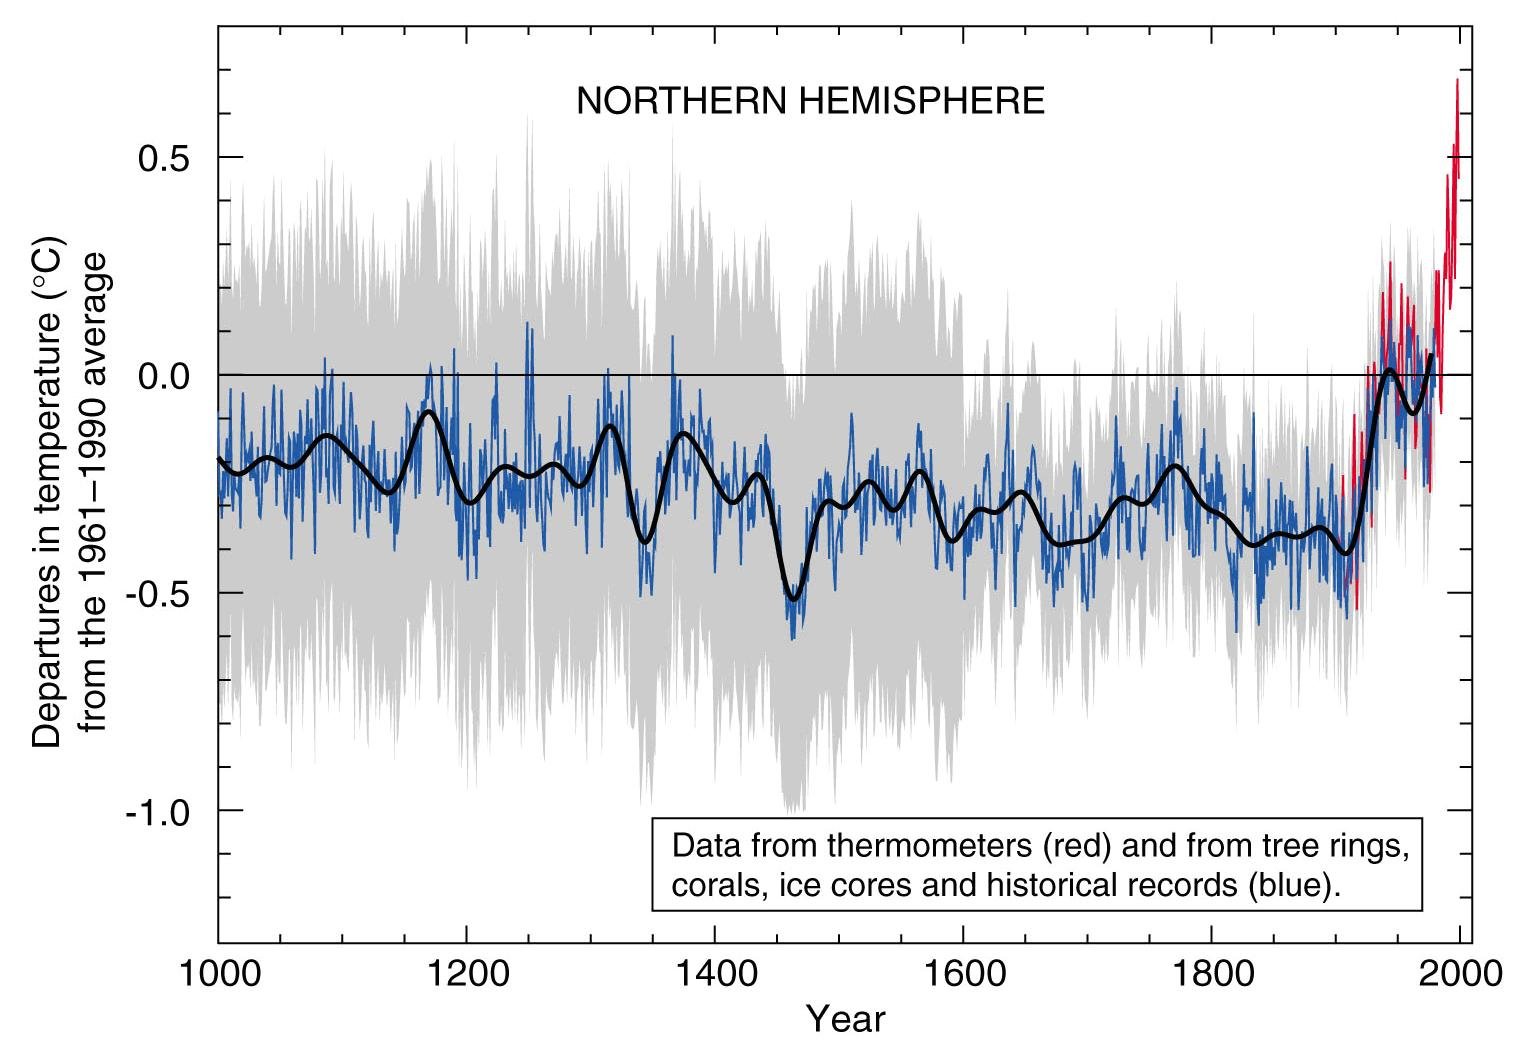
\includegraphics[width=0.99\linewidth]{img/hockey.png} 
\end{center}
\caption{Famous Hockey stick graph~\cite{mann1999northern}. (We suggest that you use graphic (which is a 300 dpi resolution TIFF, EPS, PNG or JPG.) }
\label{fig:hockey}
\end{figure}

\section{References Style}
Since 1 January 2021 we apply the IEEE Citation Style.
It is suggested for authors to use BibTex system and specialized platform for selection and writing references (for example Mendeley, Zotero or other reference manager). It is strongly recommended to provide DOI where possible~\cite{stando2020constant}.

Any citation style is set up to give the reader immediate information about sources cited in the text. In IEEE style citations, the references should be numbered and appear in the order they appear in the text. When referring to a reference in the text of the document, put the number of the reference in square brackets. 

The IEEE citation style has 3 main features:
\begin{itemize}
\item The author name is first name (or initial) and last name.
\item The title of an article (or chapter, conference paper, patent etc.) is in quotation marks.
\item The title of the journal or book is in italics.
\end{itemize}

These conventions allow the reader to distinguish between types of reference at a glance. The correct placement of periods, commas and other punctuation marks depends on the type of reference cited. Check the examples below. By using official ieeetr.bst file you can be sure that all the details are correct.

Check the distinctions between print and electronic sources (especially for journals) carefully.

Examples of citations: 
books (\verb+@book+ bibtex entry)\cite{kazmierkowski1994automatic}\cite{wilamowski2018power},
book chapters (bibtex entry \verb+@incollection+)\cite{urry2016photosynthesis}\cite{kazmierkowski2011control},
journal articles (bibtex entry \verb+@article+) \cite{mann1999northern}\cite{kaczorek2005generalization}\cite{stando2020constant}, 
conference proceedings (bibtex entry \verb+@inproceedings+)  \cite{lizotte2016multi}\cite{kocsis2006uct},
on-line sources \cite{gelly2012grand}\cite{zotero_zotero_2018}\cite{ieeetranbst}.
For other types of sources check documentation of IEEETran Bibtex style~\cite{ieeetranbst}.


\section{Conclusions}

Provided \LaTeX~ document style (bpasts.sty) and bibtex style (IEEEtran.bst) are responsible for proper formatting of your paper. The authors are encouraged to take advantage of these possibilities and avoid manual modification of formatting.

\section*{Appendix}
Appendixes, if needed, appear before the acknowledgment.

%%%%%%%%%%%%%%%%%%%%%%%%%%%%%%%%%%%%%%%%%%%%%%%%%%%%%%%
%% ACKNOWLEDGEMENTS
\begin{acknowledgements}
Avoid the stilted expression “one of us (R. B. G.) thanks ...”.  Instead, try “R. B. G. thanks...”. Put sponsor acknowledgements unnumbered at the end of the text and before References.
\end{acknowledgements}

%%%%%%%%%%%%%%%%%%%%%%%%%%%%%%%%%%%%%%%%%%%%%%%%%%%%%%%
%% REFERENCES
%% Since January 1st 2021, IEEE Citation Style should be applied.
%\bibliographystyle{IEEEtran}
\bibliographystyle{IEEEtranUrldate}

%% Change to your *.bst file
\bibliography{sampleBibFile}

\end{document}


